\noindent All of the haematocrits reported are discharged haematocrits, H$_{D}$, and it is calculated as the ratio of RBC flux to blood flow rate (Equation \ref{HaematocritEqn}) in each selected branch across the microvascular network. The volumetric blood flow is determined by integrating the blood velocity with respect to the cross- sectional area of the branch normal to the direction of blood flow. $Q_{rbc}$ represents the volumetric flow rate of RBCs while $Q_{blood}$ represents the volumetric flow rate of blood.

\begin{eqnarray}
\label{HaematocritEqn}
\begin{aligned}
H_{D} & = \frac{Q_{rbc}}{Q_{blood}}
\end{aligned}
\end{eqnarray}

\bigskip

\noindent The volumetric flow rate of RBC is calculated by counting the number of RBCs ($N$) crossing the same plane normal to the direction of blood flow over a given period of time, $\Delta t$. In order to satisfy mass conservation, the counting procedure is conducted when the total number of RBCs in the simulated network has become quasi-constant. Hence, given that the volume of an RBC is known (V$_{rbc}$ $=$ 100 $\mu$m$^{3}$), we can then calculate the RBC flow rate using Equation \ref{RBCflowrateEqn} below. 

\begin{eqnarray}
\label{RBCflowrateEqn}
\begin{aligned}
Q_{rbc} & = \frac{N \cdot V_{rbc}}{\Delta t}
\end{aligned}
\end{eqnarray}

\bigskip

\noindent The flow resistance ($R$) is evaluated from simulation data using the left-hand side (LHS) of the Hagen-Poiseuille's Equation\cite{PoiseuilleLaw} (Equation \ref{HagenPoiseuilleEqn1}) where direct measurements of blood flow rate ($Q_{blood}$) and pressure drop ($\Delta$P) for each branch are obtained via ParaView and Python. $\Delta$P is calculated by taking the difference between measured pressures at the start and endpoints of each branch. 

\begin{eqnarray}
\label{HagenPoiseuilleEqn1}
\begin{aligned}
R & = \frac{\Delta P}{Q} = \frac{128L\mu_{app}}{\pi D^{4}}
\end{aligned}
\end{eqnarray}

\bigskip

\begin{figure}[H]
\centering
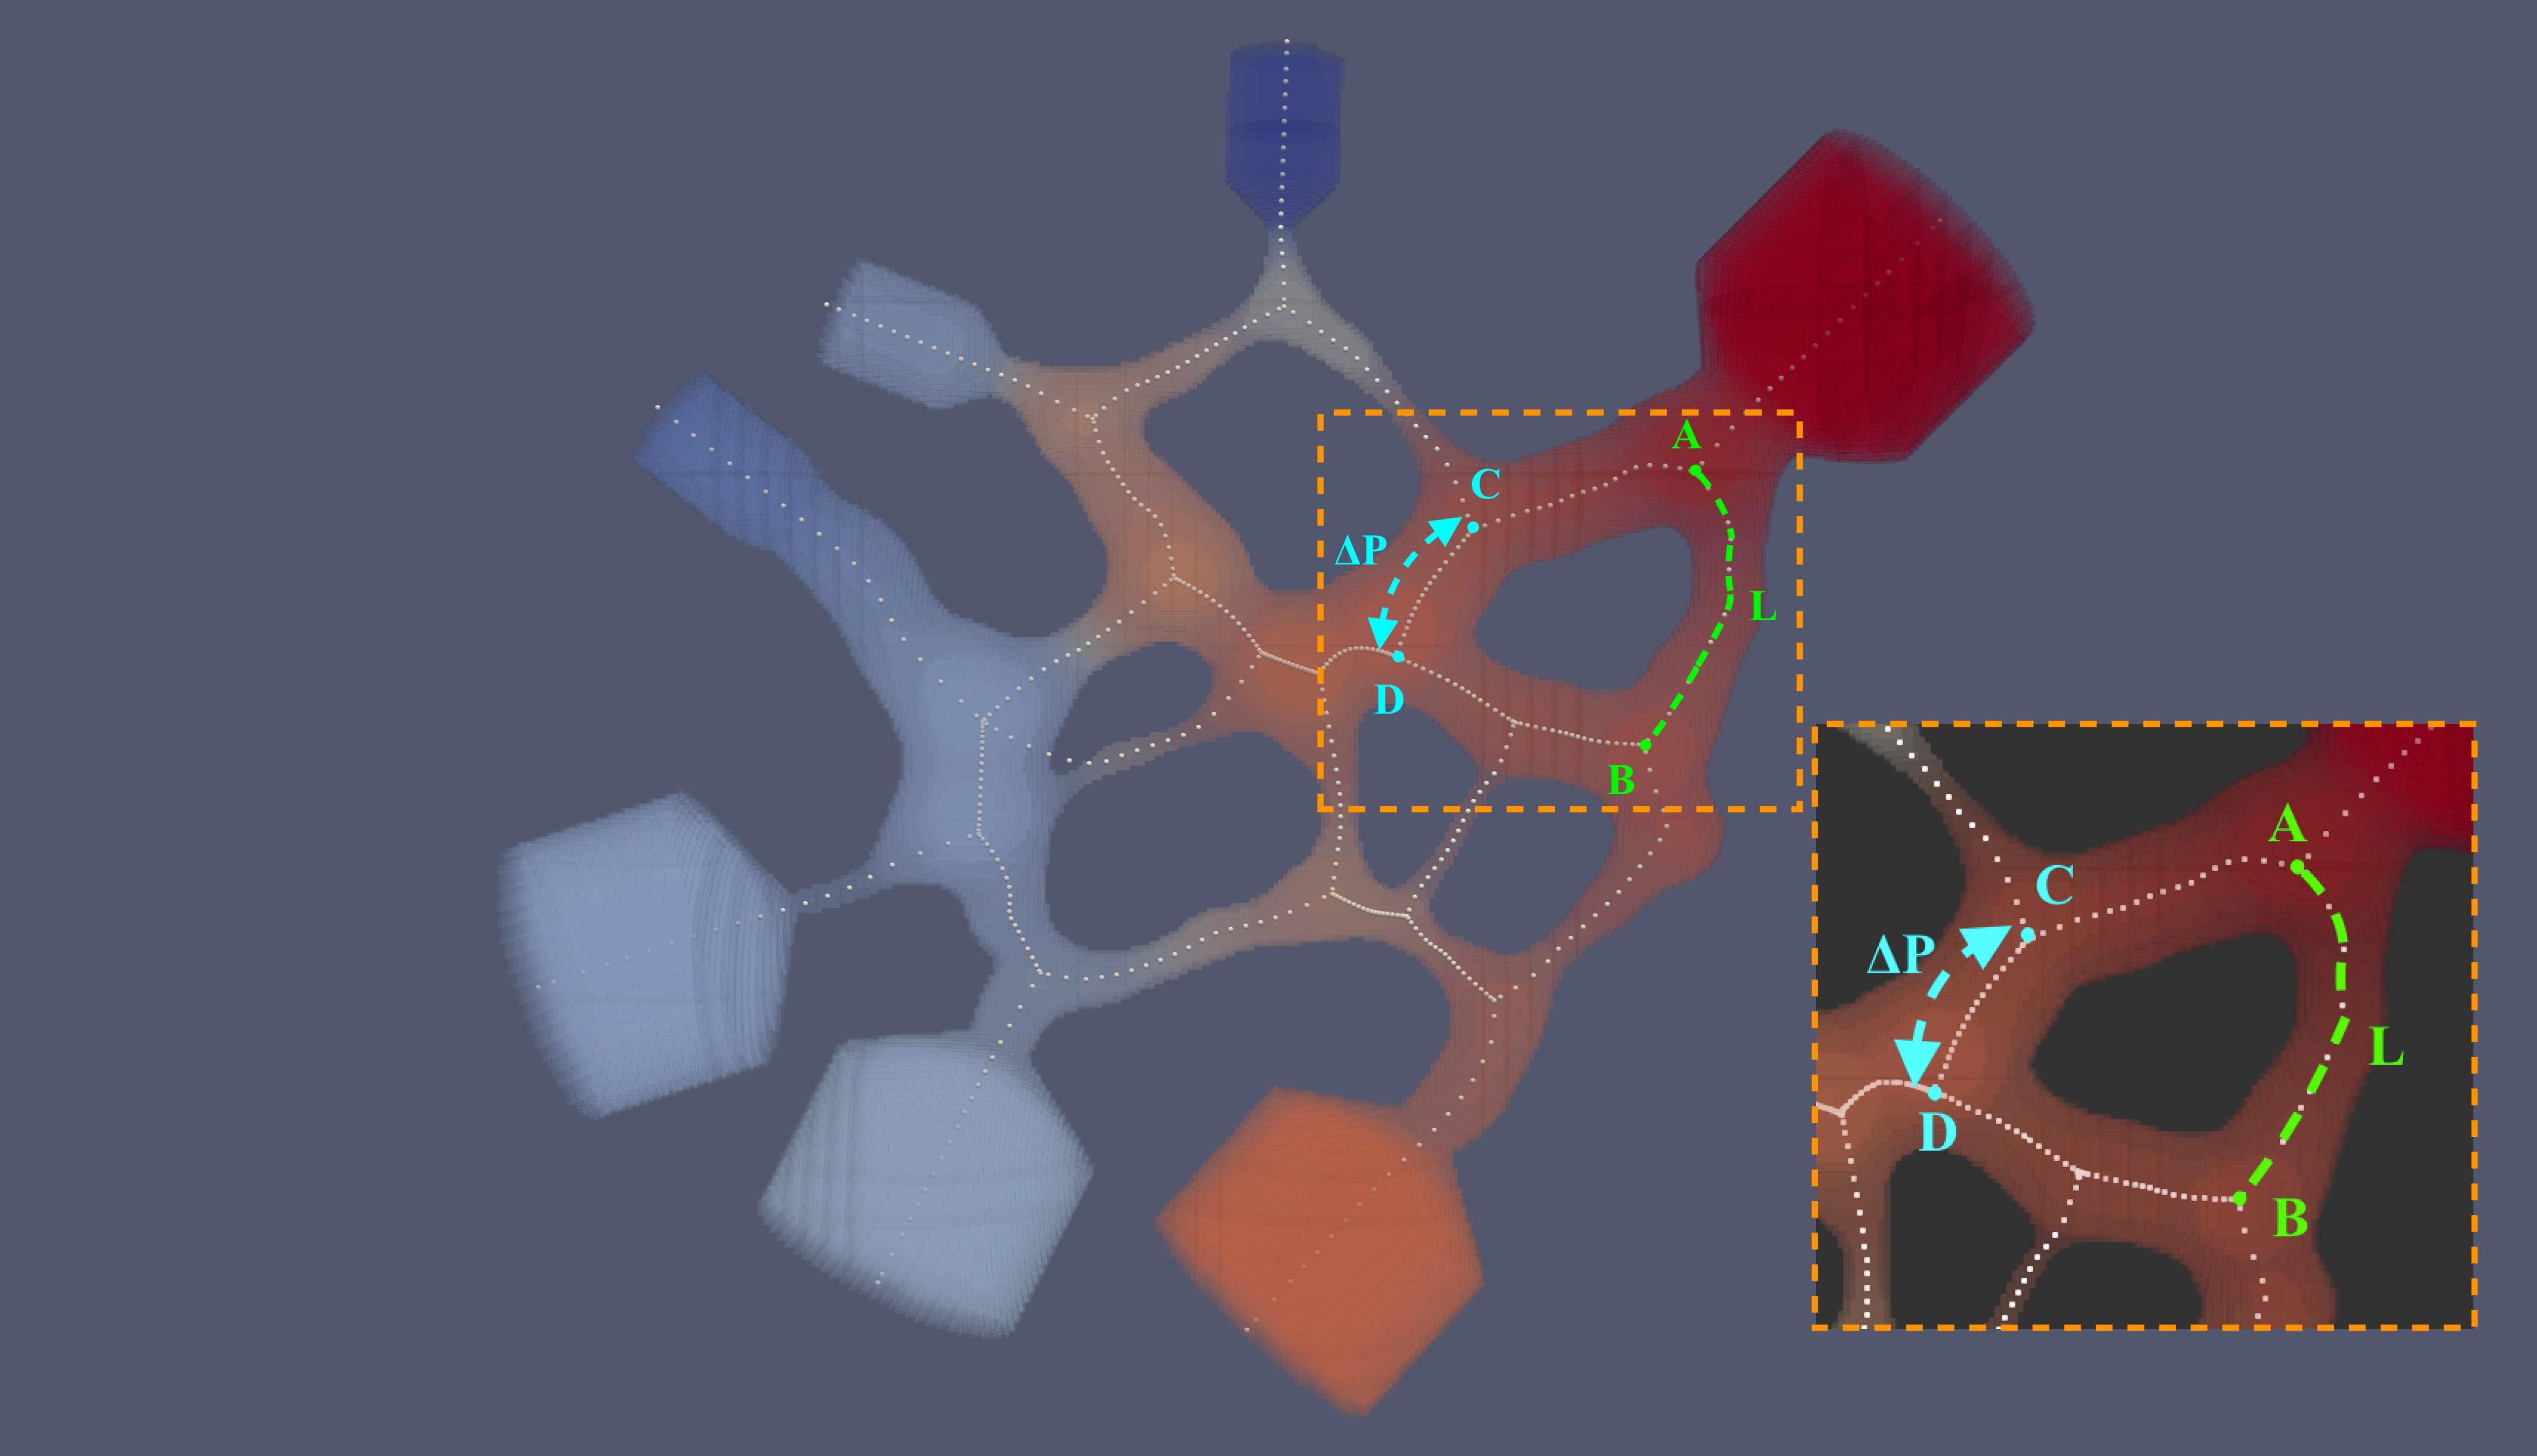
\includegraphics[width=1\textwidth]{images/ROI3-Geometry.png}
\caption{\textit{A complex micro-vascular network with an illustration of the measurement methods for pressure drop across the branch and branch length.} \label{measurementmethods}}
\end{figure}

\noindent Morphological variables such as the geometric diameter (D$_{G}$) and branch length ($L$) are measured as well based on the ROI geometries. D$_{G}$ is calculated by averaging all of the diameter measurements within a given vessel segment. Whereas for $L$, the distance between two points within a vessel is first measured before adding up all of the measured distances in the given vessel to obtain the magnitude of the branch length. In addition to this, the hydrodynamic diameter (D$_{H}$) of each branch is calculated using the Hagen-Poiseuille's Equation with the plasma-only simulation data. An illustration of the measurement methods is shown in Figure \ref{measurementmethods}. \\

\noindent Although the viscosity of blood flowing through micro-vessels is usually not constant, a simplified approach is used to obtain the apparent viscosity of blood (i.e. plasma+RBC) from simulation data. This is achieved by rearranging Equation \ref{HagenPoiseuilleEqn1} to Equation \ref{HagenPoiseuilleEqn2}. Therefore, it also allows us to conveniently analyse the rheological effects associated with RBCs in micro-vessels from simulation data. The relative apparent viscosity is defined as $\mu_{rel} = \mu_{app}/\mu_{p}$, where $\mu_{p}$ is the viscosity of suspending medium (i.e. plasma). A comparison is also made between the evaluated apparent viscosity values based on either geometric (D$_{G}$) or hydrodynamic (D$_{H}$) diameters in order to determine which is the preferable input parameter for apparent viscosity estimations. 


\begin{eqnarray}
\label{HagenPoiseuilleEqn2}
\begin{aligned}
\mu_{app} & = \frac{\pi}{128} \cdot \frac{\Delta PD^{4}}{LQ}
\end{aligned}
\end{eqnarray}

\bigskip

\noindent Since one of the most distinguished characteristics of micro-circulatory blood flow is the disproportionate partitioning of RBCs at vascular diverging bifurcations, the time-averaged behaviours of RBC partitioning are considered in the data analysis. Based on the studies from Pries et al.\cite{PRIES198981} and Balogh and Bagchi\cite{Balogh2018}, the ratio of blood flow rates (Q$^{*}_{blood}$) and RBC flux ratio (Q$^{*}_{rbc}$) between a child branch and the parent branch of each bifurcation are calculated using Equations \ref{Qratio1} and \ref{Qratio2} respectively as shown below.

\begin{eqnarray}
\label{Qratio1}
\begin{aligned}
Q^{*}_{blood} & = \frac{Q_{blood,CB}}{Q_{blood,PB}} 
\end{aligned}
\end{eqnarray}

\begin{eqnarray}
\label{Qratio2}
\begin{aligned}
Q^{*}_{rbc} & = \frac{Q_{rbc,CB}}{Q_{rbc,PB}} 
\end{aligned}
\end{eqnarray}